% !TeX root = ..

\section{
  Задача маршрутизации перемещений
  (частная~постановка~задачи)
}
\label{sect:5.2}
\setcounter{equation}{0}

В настоящем разделе мы следуем конструкциям главы~3
и рассматриваем далеко не самый общий случай постановки,
ориентированной на применение в задаче маршрутизации
движения инструмента при листовой резке на машинах с ЧПУ.
Содержательное обсуждение задачи приведено в главе~3
и в первой части монографии.
Сейчас мы остановимся только на одном моменте,
связанном с ограничениями,
придерживаясь содержательного способа изложения.


Как и в главе~3,
мы полагаем заданными мегаполисы
$M_1,\,\ldots,M_N,$
которые в нашей конкретной задаче являются непустыми конечными множествами на плоскости,
располагающимися на некоторых <<вторичных>> эквидистантах.
Имеются отношения
$\bbm_1,\,\ldots,\bbm_N;$
при этом $\bbm_j\subset M_j\times M_j.$
Элементами
$\bbm_j,$ где $j\in \ov{1,N},$
являются упорядоченные пары $(x,y),$
где $x$ --- возможная точка врезки,
а $y$ --- точка выключения инструмента;
разумеется, $x$
и $y$ --- суть плоские векторы.
В этой связи отметим, что в качестве объемлющего
множества $X$ далее используется плоскость:
$$
  X = \bbr\times \bbr
  .
$$

В качестве $X$
может использоваться также достаточно большой прямоугольник на плоскости.
Сохраняем определения множеств
$\mathbf{M}_1,\,\ldots,\mathbf{M}_N, \bbx$
и $\mathbf{X},$
которые были введены в главе~3.
В настоящем разделе предполагаем заданными операторы (\ref{3.3.9});
каждый из этих операторов сопоставляет точке множества $\mathbf{X}$
непустое конечное множество на плоскости,
причем, как уже отмечалось в главе~3
(см. замечание после (\ref{3.3.11}))
в определении $A_1,\,\ldots,A_N$
допускается определенная избыточность;
существенная <<часть>> данных определений
для одного из возможных вариантов реализована в замечании~\ref{z3.3.2}.

В непосредственных расчетах использовался несколько иной вариант определения
$A_1,\,\ldots,A_N$
(ограничиваемся определением значений, существенных для рассматриваемой маршрутной задачи).
Пусть
$$
  \rho:\,X\times X \longrightarrow [0,\infty[
$$
есть обычная евклидова метрика на $X;$
при
$x_1\in X$ и $x_2\in X$
число
$$
  \rho(x_1,x_2)\in [0,\infty[
$$
определяет евклидово расстояние между плоскими векторами
$x_1$ и $x_2.$
Рассмотрим нужный вариант, фиксируя
$j\in\ov{1,N}$ и полагая
(это достаточно для всех наших целей), что
$x\in \mathbf{X}\setminus \mathbf{M}_j.$
По самому смыслу оператора $A_j$ (\ref{3.3.9})
имеем, что множество $A_j(x)$
исчерпывает возможности выбора новой точки врезки при
условии перемещения в мегаполис из состояния $x,$
которое не принадлежит
$\mathbf{M}_j$:
мы имеем возможность выбирать только векторы $y\in A_j(x).$
Одно из соображений, определяющих упомянутое ограничение,
может состоять в том,
чтобы новая точка врезки выбиралась в отдалении от предыдущей.
Здесь,
конечно, надо иметь в виду, что реально у нас либо
$x=x^o,$ либо $x$ является
точкой выключения инструмента и может не совпадать с предыдущей точкой врезки.
Однако в рассматриваемой задаче <<парные>> точка врезки и точка выключения
(инструмента) близки,
а потому можно считать, что предыдущая точка врезки находится вблизи
$x$ и, отдаляясь от $x,$
мы удаляемся и от упомянутой предыдущей точки врезки.

Будем полагать заданным некоторое число
$\mathbf{r}_j(x)\in [0,\infty[$
(пороговый уровень)
и весовой коэффициент
$\xi_j(x) \in ]0,1]$.
Введем значение
$$
  d_j(x) \df \max\limits_{h\in \bbm_j}\rho\bigl(x,\mathrm{pr}_1(h)\bigl)
  ,
$$
в нашем случае
$d_j(x) > 0$.
Определяем множество $A_j(x)$ следующими тремя выражениями:
$$
  \bigl(d_j(x) < \mathbf{r}_j(x)\bigl)\Longrightarrow \Bigl(A_j(x) \df
  \bigl\{\mathrm{pr}_1(y):\,y\in \bbm_j,\ \xi_j(x) d_j(x) \leqslant \rho
  \bigl(x,\mathrm{pr}_1(y)\bigl)\bigl\}\Bigl)
  ,
$$
$$
  \biggl(\Bigl(\min\limits_{h\in \bbm_j}\rho\bigl(x,\mathrm{pr}_1(h)\bigl)
  \leqslant \mathbf{r}_j(x)\Bigl)\,\&\,\bigl(\mathbf{r}_j(x)\leqslant d_j(x)
  \bigl)\biggl) \Longrightarrow $$ $$\Longrightarrow\Bigl(A_j(x) \df \bigl
  \{\mathrm{pr}_1(z):\,z\in \bbm_j,\ \mathbf{r}_j(x) \leqslant \rho\bigl(x,
  \mathrm{pr}_1(z)\bigl)\bigl\}\Bigl)
  ,
$$
$$
  \Bigl(\mathbf{r}_j(x) < \min\limits_{h\in\bbm_j}\rho\bigl(x,
  \mathrm{pr}_1(h)\bigl)\Bigl)\Longrightarrow \bigl(A_j(x) \df
  \{\mathrm{pr}_1(h):\,h\in \bbm_j\}\bigl)
  .
$$

В первом из соотношений говорится о <<хоть каком-то>> уклонении от предыдущей
точки врезки
(число $\xi_j(x)$ логично выбирать близким к 1).
Речь идет об обработке <<плохих>> в упомянутом смысле случаев.
Второе соотношение
характеризует пороговое разделение множества новых точек врезки на два подмножества,
одно из которых и трактуется как $A_j(x).$
Наконец, третье соотношение отвечает <<хорошему>> в смысле упомянутой удаленности случаю,
когда любые точки врезки нового мегаполиса доступны для перемещения.

Заметим, что упомянутое <<тройственное>> определение обеспечивает условие
$A_j(x) \neq \emp,$
хотя при $d_j(x) < \mathbf{r}_j(x)$
за это условие приходится <<расплачиваться>> качеством реализации порогового уровня
$\mathbf{r}_j(x);$
по сути дела мы действуем в случае упомянутого строгого
неравенства по остаточному принципу.
Тем не менее определенные меры в части
осуществления удаленности новой точки врезки от предыдущей удается реализовать
и обеспечить тем самым постановку задачи (\ref{3.3.31})
в ее конкретном варианте.

При построении алгоритма использовались соглашения:
$$
  \bigl(\mathbf{r}_j(x) = \mathbf{r}\ \ \fa j\in \ov{1,N}\ \ \fa x\in
  \mathbf{X}\setminus \mathbf{M}_j\bigl)\,\&\,\bigl(\xi_j(x) = \xi\ \ \fa
  j\in \ov{1,N}\ \ \fa x\in \mathbf{X}\setminus \mathbf{M}_j\bigl)
  .
$$
Напомним, что при доопределении вышеупомянутых <<тройственных>> правил до
отображений на всем множестве $\mathbf{X}$ использовались соображения,
подобные изложенным в \ref{sect:3.3}
после соотношения (\ref{3.3.11});
здесь $\mathbf{r}>0$
и $1 \geqslant\xi >0$.

Рассматриваемые в книге примеры связаны с машинами резки металла на станках с ЧПУ.
Функции стоимости представляют собой не расстояния,
а времена движения инструмента.
Все перемещения осуществляются либо на скорости холостого хода $V_i,V_i>0$,
либо на скорости реза
$V_c, V_c > 0$.
Скорость холостого хода превышает скорость
реза в десятки и сотни раз.
В примерах $V_i=500$ мм/с, а $V_c=10$ мм/с.
Движение предполагается безынерционным.
Точка $x^0$ задается в виде начала координат:
$x^0=(0,0)$.
Для
$x_1\in \mathbf{X}$ и
$x_2\in \mathbb{X}$ полагаем
\begin{equation}
  \label{ExtPrice}
  \mathbf{c}(x_1,x_2)=\frac{\rho (x_1,x_2)}{V_i}
  .
\end{equation}

Функции стоимости внутренних работ вычисляются с учетом скорости реза.
Именно для
$i\in \overline{1,N}$, $z\in \mathbb{M}_i$
$$
  c_i(z)=\frac{\rho(\mbox{pr}_1(z),u(z))+\rho(u(z),\mbox{pr}_2(z))}{V_c}
  ,
$$
где вектор $u(z)$
находится на эквидистанте и сопоставляется $z$ однозначно.
Функция $f$
также определяется временем движения в финишную точку
\begin{equation}
  \label{TerminalPrice}
  f(x)=\frac{\rho (x,x^0)}{V_i}
  .
\end{equation}
%^^^^^^^^^^^^^^^^^^^^^^^^^^^^^^^^^^^^^^^^^^^^^^^^^^^^^^^^^^^^^^^^^^^^^^^^^^^^^^^

%*******************************************************************************
В примере,
изображенном на рис.~\ref{DP_Result},
рассматривался случай
\mbox{$N=29$} и
$|\mathbf{K}| =30$.
Использовалось <<тройственное>> определение операторов
$A_1,\,\ldots,A_N$
при следующей конкретизации параметров:
$$
  \mathbf{r}=100,\ \xi=0,75
  .
$$

\begin{figure}[H]
  \centering
  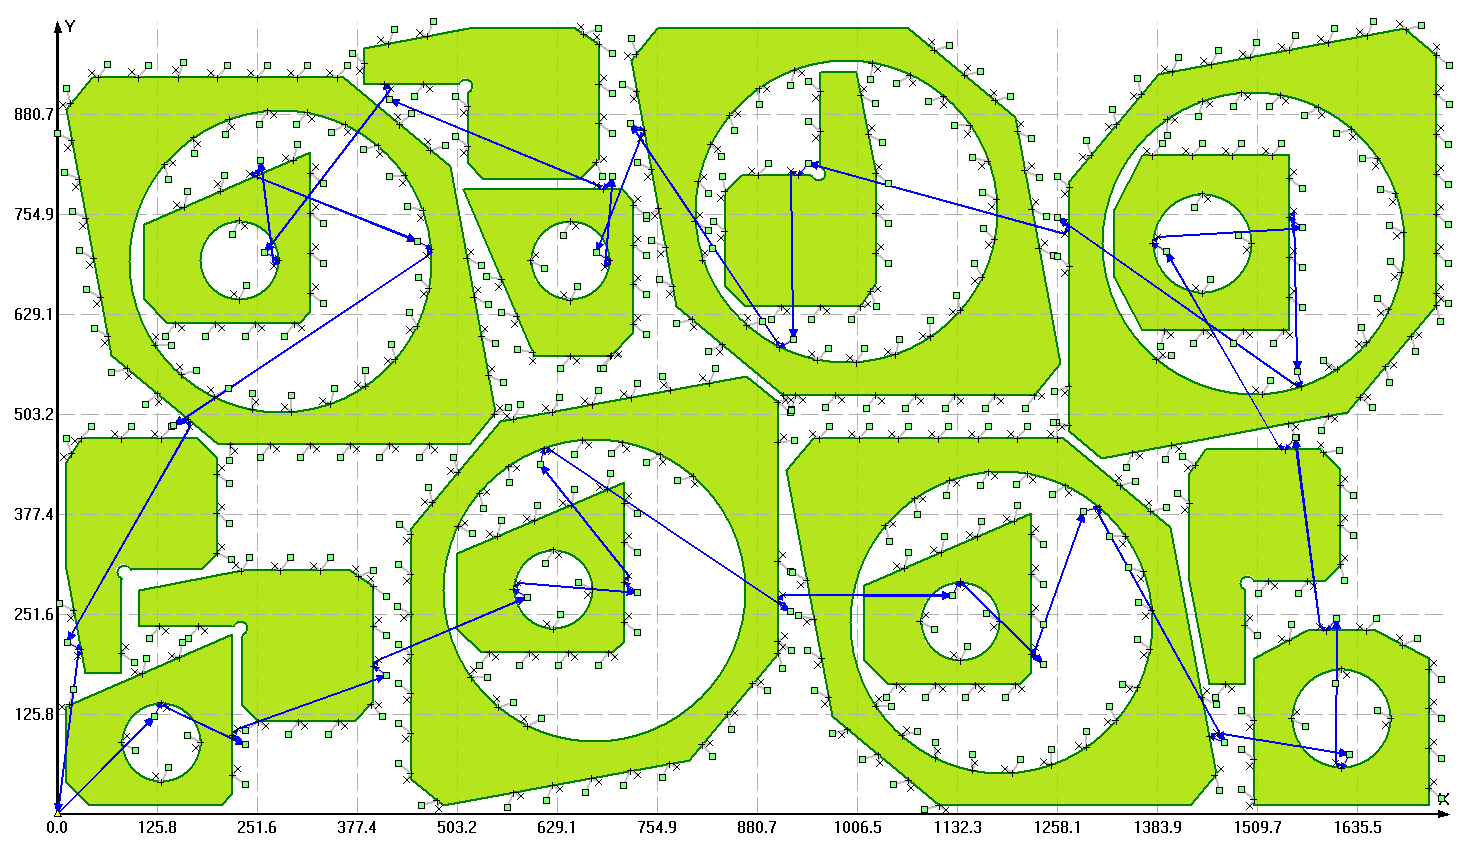
\includegraphics[width=0.9\textwidth]{route_29_DP_AD.png}
  \caption{
    Траектория, построенная на основе ДП
  }
  \label{DP_Result}
\end{figure}

Точное описание мегаполисов не приводится по соображениям объема.
Отметим только, что мощности
$|M_i|, i\in \overline{1,29}$,
имеют значение от 3 до 30.

Результат счета 100,61,
время счета 13 мин 13 с.
Маршрут и трасса показаны
на рис. \ref{DP_Result}.
